\documentclass[a5paper,12pt]{article}
\usepackage[utf8]{inputenc}
\usepackage[IL2]{fontenc}
\usepackage{listings}
\usepackage{amssymb}
\usepackage{amsmath}
\usepackage{url}
\usepackage{graphicx}
\usepackage[czech]{babel}
\usepackage[landscape]{geometry}
\title{Teorie her}
\author{Michal Abaffy, Marek Bryša, Jan Kovář}
\date{Brno, \today}
\begin{document}
  \maketitle
  \section{Úvod}
  \section{Aplikace v ekonomických experimentech}
    \subsection{Hra diktátor}
      \emph{Diktátor} je nejjednodušší možná hra nebo spíše situace individuálního rozhodnutí,
      která může osvětlit preference ohledu na druhé. Tato hra má dva hráče: navrhovatele a příjemce.
      Navrhovatel rozhodne, jak se má rozdělit obdaření dané velikosti mezi něho a příjemce,
      což se pak také stane. Role příjemce je čistě pasivní.

      Implementace v laboratoři může vypadat takto: obdaření \$10 je poskytnuto experimentátorem jako
      \uv{dar z nebes}. Testované subjekty jsou náhodně náhodně rozděleny mezi navrhovatele a příjemce.
      Anonymita rozhodnutí a párování je zaručena.
        
      Tento experiment byl poprvé uveden v Forsythe et al. (1994) s těmito výsledky:
      \begin{itemize}
        \item
          Je zjevné, že mnoho subjektů se nechová zcela sobecky, což odporuje konvenční teorii založené na
          ohledech na sebe.
        \item
          Tento výsledek byl od té doby mnohokrát ověřen. Typicky více než 60\% subjektů předá kladnou částku,
          průměrné 20\% obdaření. Toto je však velmi závislé na procedurálních detailech, viz dále.
      \end{itemize}
      Cherry et al. (2002) říka, že pokud je obdaření nutno \uv{vydělat} např. tak, že navrhovately se stali ti,
      kteří uspěli ve vědomostním kvízu, převod kladných částek prakticky vymizí. (zde byla anonymita zaručena i
      vůči experimetátorovi)
      
      List (2007) ukazuje, že pokud je navrhovateli navíc dána možnost vzít peníze příjemci, prevod kladných částek
      opět zmizí a nejčastějším návrhem se stane sebrání co nejvíc peněz od příjemce. Pokud dále je obdaření vyděláno,
      přibližne 70\% navrhovatelů neprovode žádný převod, zbytek opět sebere, co může.\\
      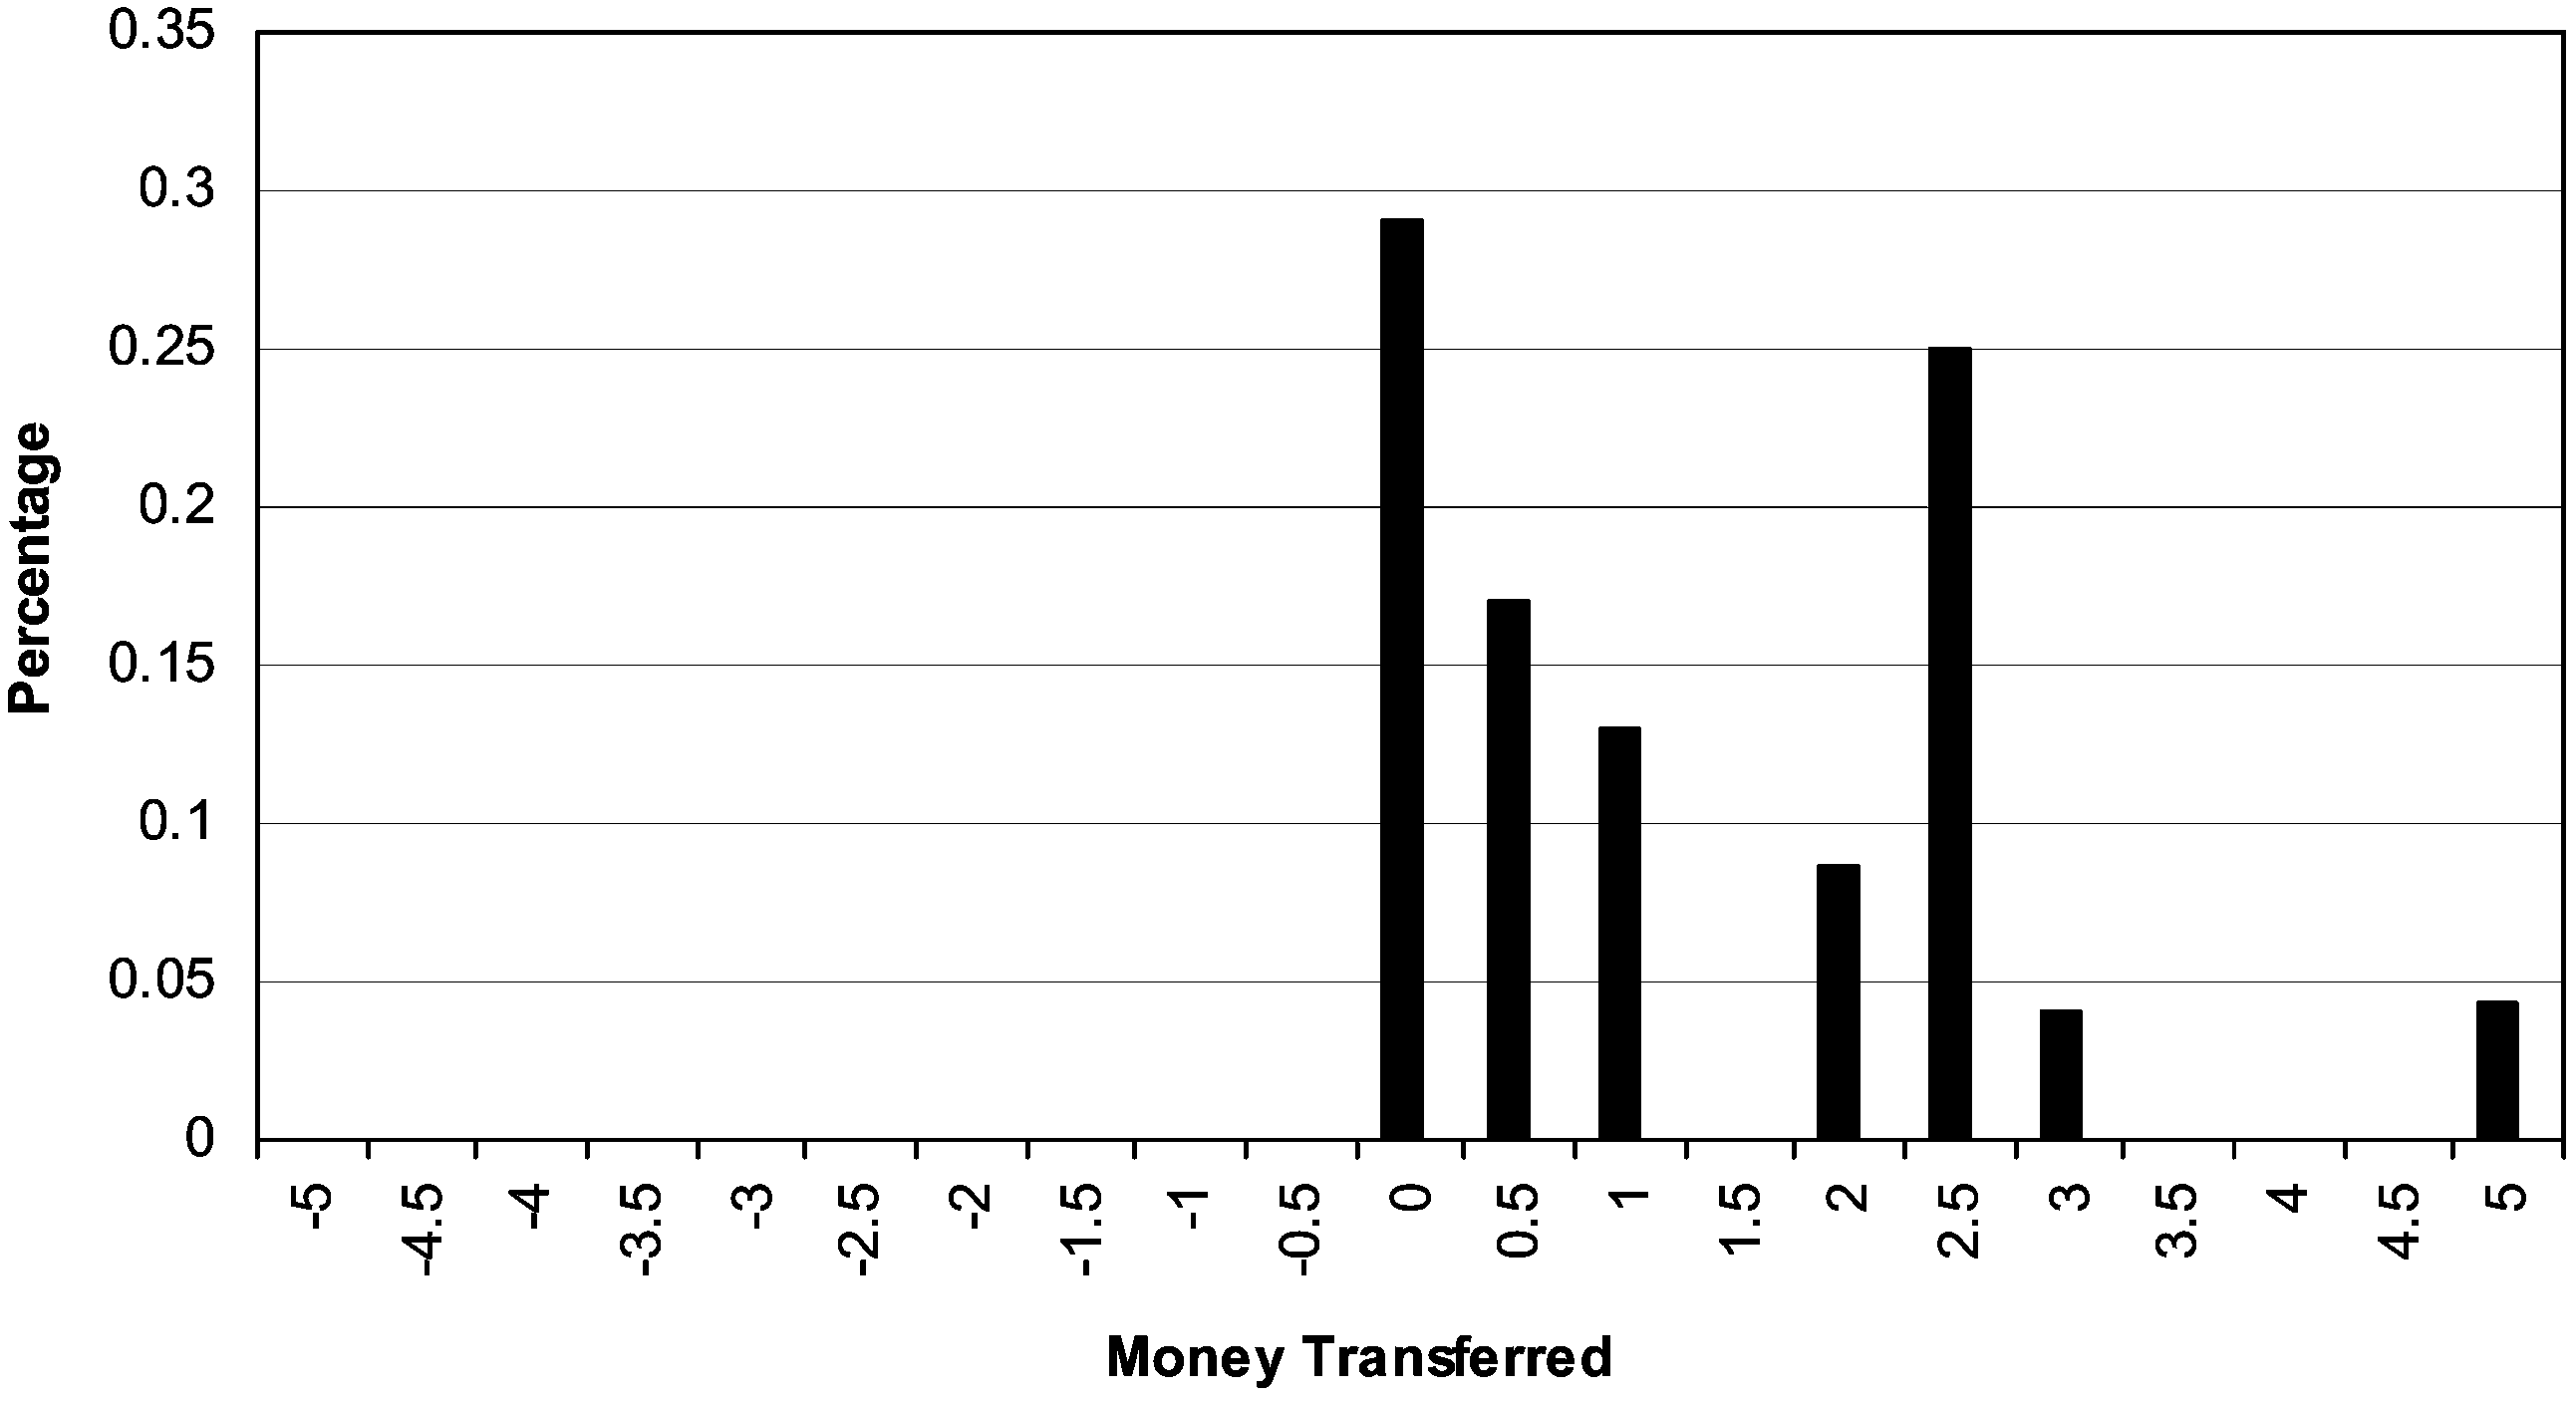
\includegraphics[width=0.5\textwidth]{list1.png}
      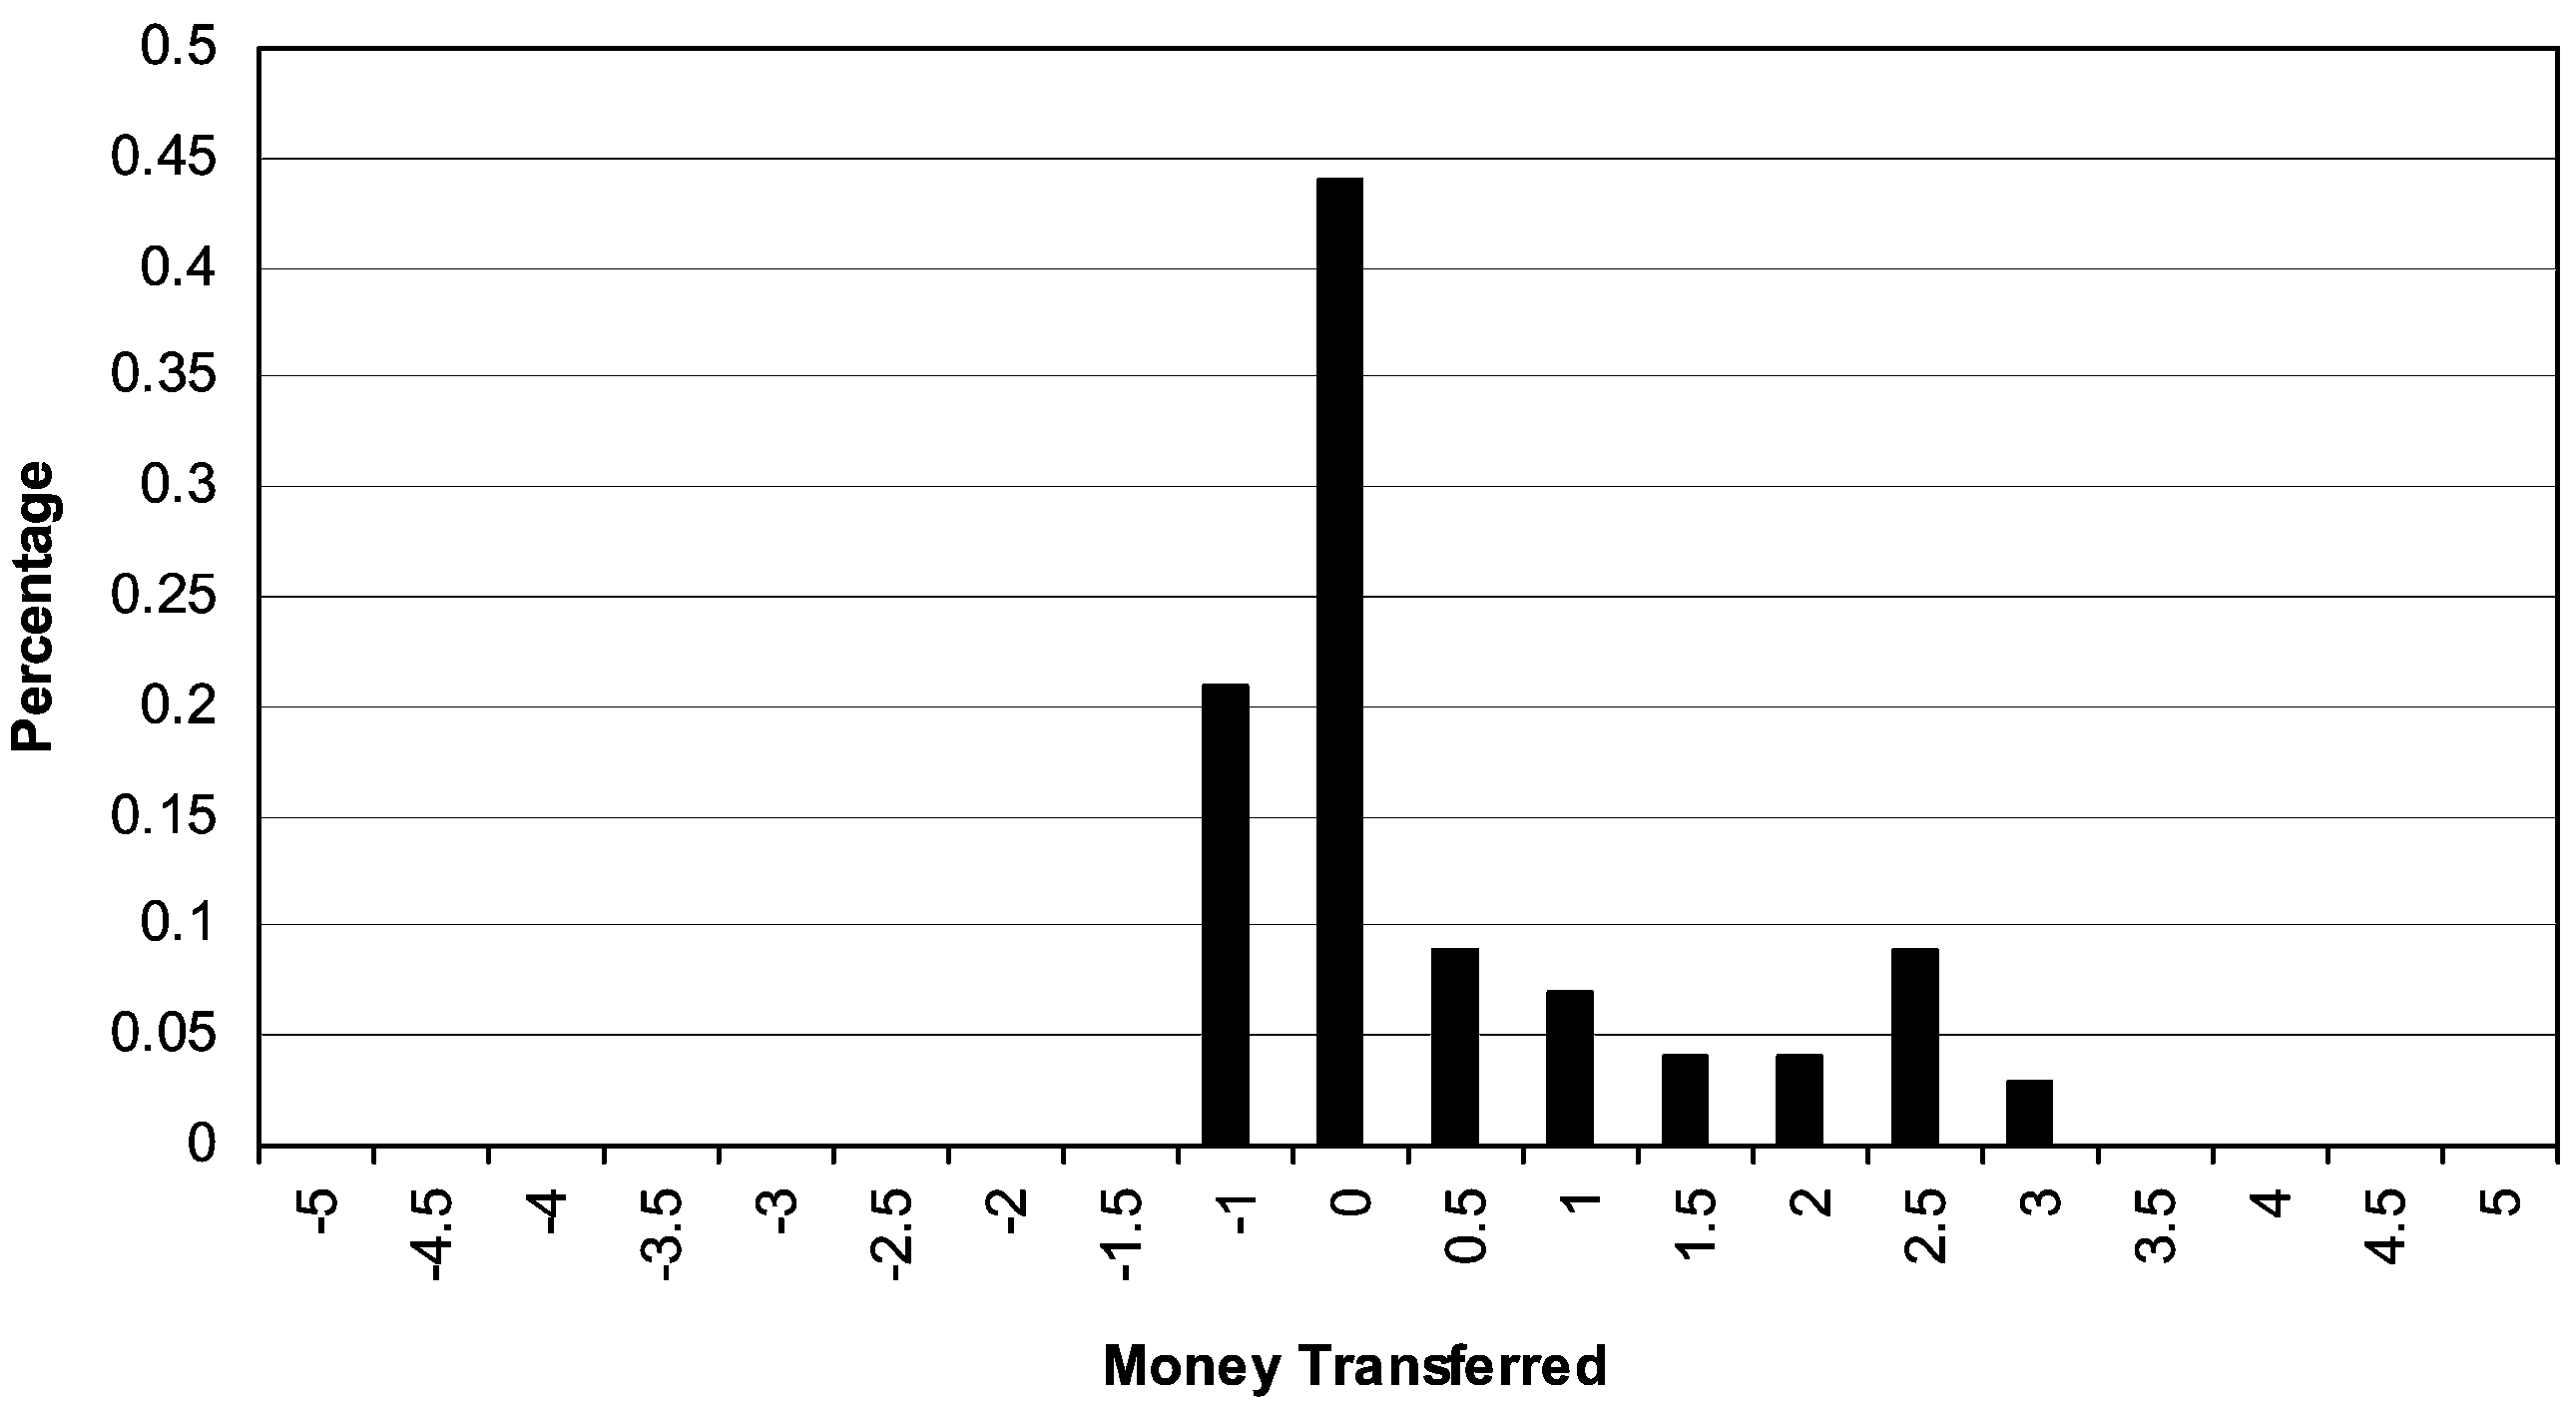
\includegraphics[width=0.5\textwidth]{list2.png}\\
      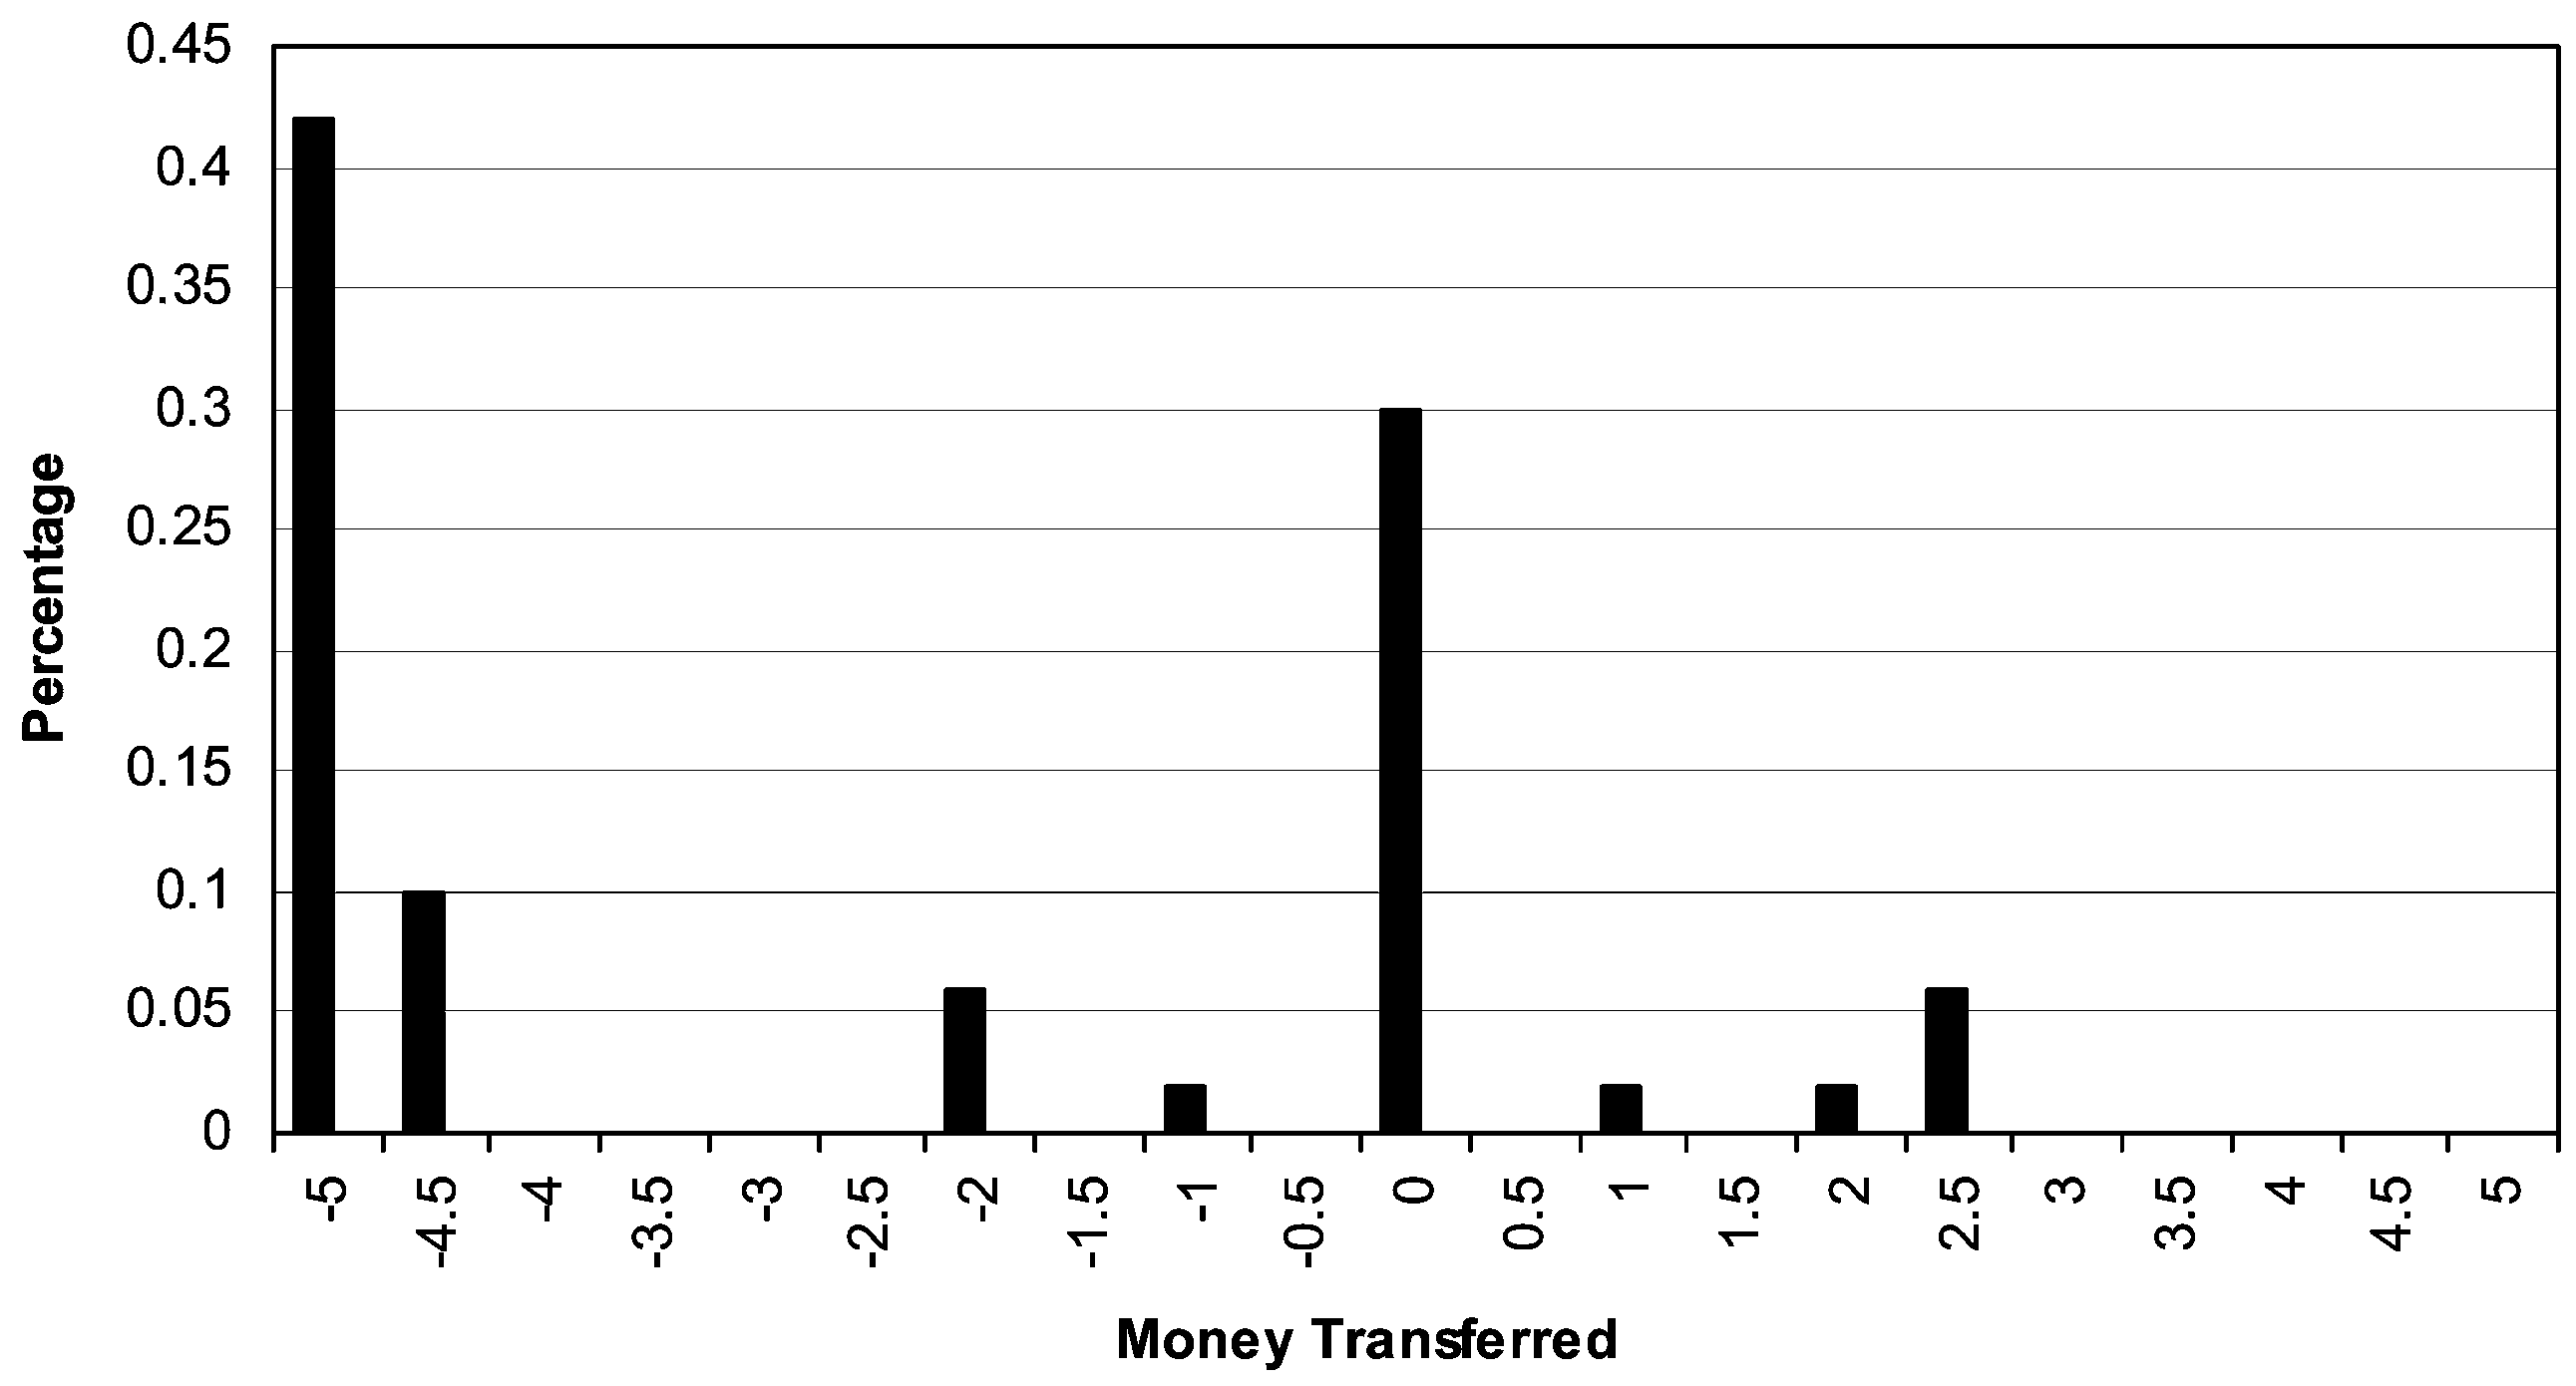
\includegraphics[width=0.5\textwidth]{list3.png}
      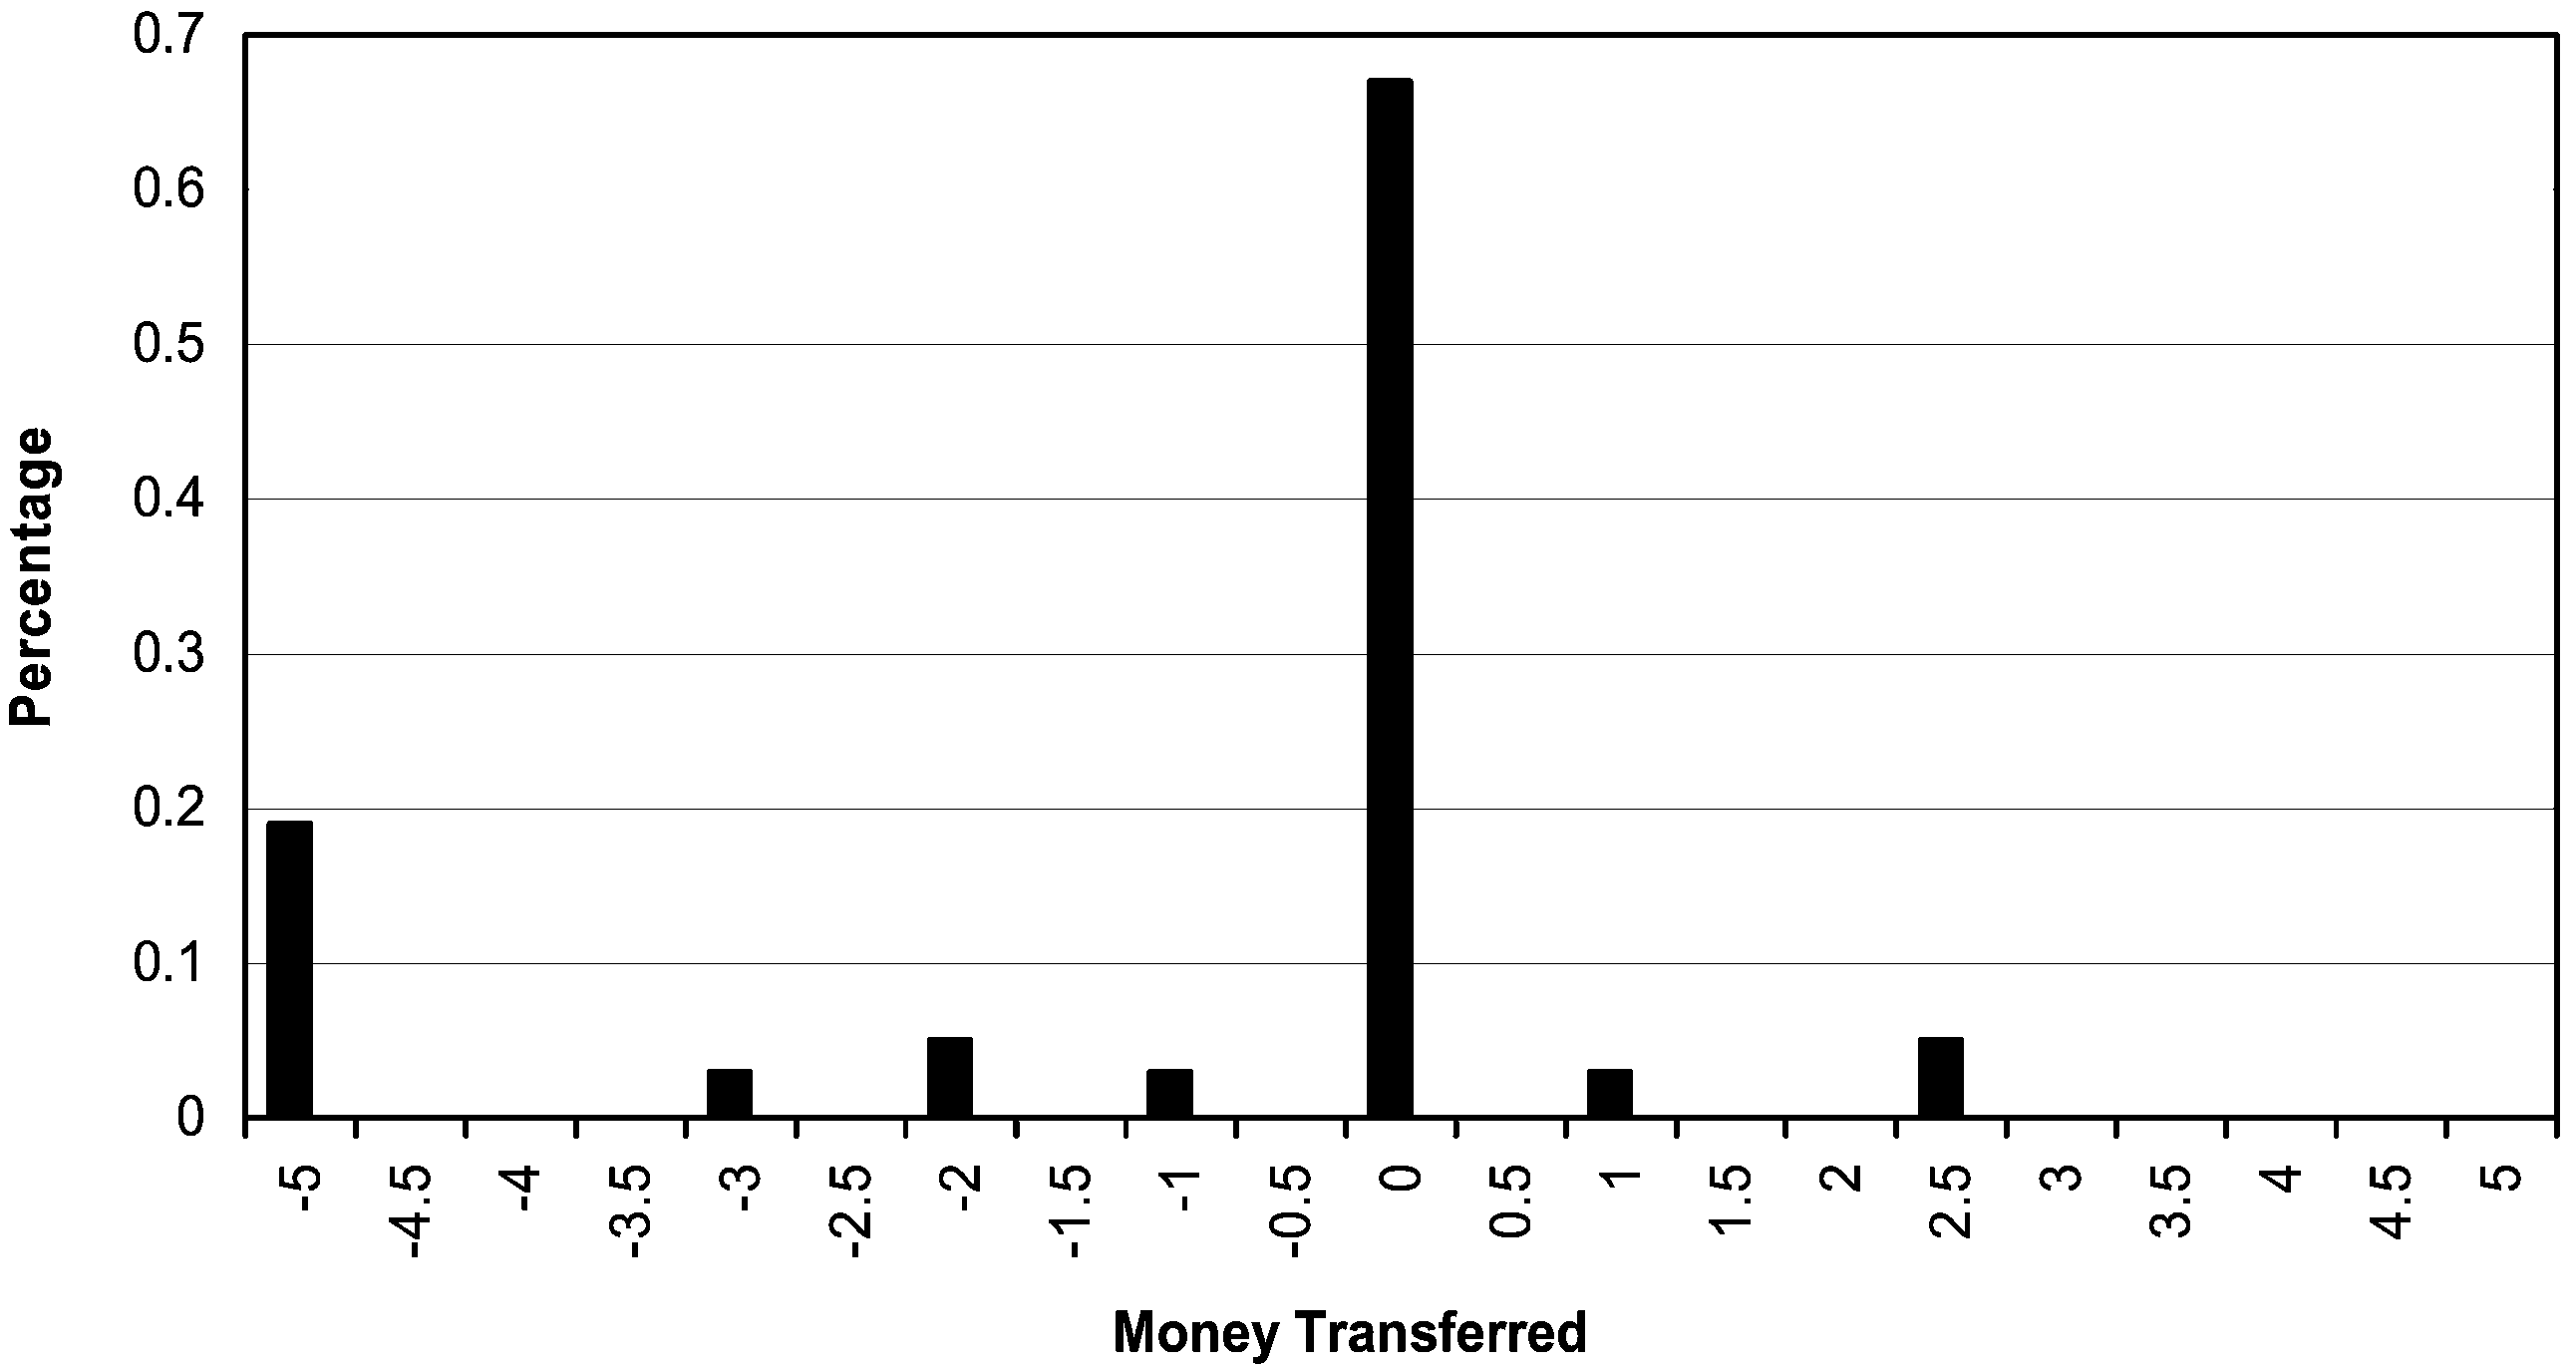
\includegraphics[width=0.5\textwidth]{list4.png}\\
    \subsection{Vyjednávání s ultimátem}
      Tato hra rozšiřuje hru \emph{Diktátor} o druhou fázi, ve které přijemce může buď akceptovat návrh rozdělení
      obdaření, nebo ho odmítnout, což znamená, že nikdo nedostane nic. Poprvé ji uvedl Guth et al. (1982).
      V této hře je příjemci dána nějaká strategická síla k ovlivnění výsledku rozdělení.
      Z předpokladu sobeckosti a použitím subgame-perfect rovnováhy vychází, že navrhovatel nabídne co nejmenší
      možnou částku a příjemce ji akceptuje, protože něco je lepší než nic.

      To se nicméně v laboratoři nepotvrdilo. Typickým výsledkem v rozvinutých zemích je nejčastější
      nabídka 40-50\% obdaření, téměř žádné nabídky nad 50\%, málo nabídek 20-40\%, které jsou v polovině
      případů zamítnuty. Zjevně empirické výsledky neodpovídají teoretickým přepokladům.

      Existuje však vysoká citlivost na detaily provedení:
      \begin{itemize}
        \item 
          Hoffman et al. (1994): 
          představení hry jako obchodní transakce místo rozdělení daru znamená pokles nejčastějšího návrhu na 40\%.
        \item 
          Pokud jsou role navrhovatele a příjemce rozděleny podle objektivního kritéria výkonu (kvíz, zručnost), 
          klesá nejčastější návrh na 30\%.
        \item
          Bornstein, Yaniv (1998):
          Pokud se rozhodují skupiny po 3-7 lidech je nejčastější návrh 35\% oproti 44\% v případě individuálního
          rozhodování za jinak stejných okolností.
        \item
          Slonim, Roth (1998):
          Čím vyšši je velikost obdaření, tím nižší je procentní návrh a ten je pravděpodobněji akceptován.
          To znamená, že příjemce se rozhoduje spíše podle absolutní hodnoty návrhu. Např. přijme 1\% z \$1000=\$10,
          ale ne 1\% z \$10=\$0.1.

      \end{itemize}
    \subsection{Dvoukrokové vyjednávání}
      Navrhovatel navrhne částku, příjmece může ihned akceptovat, nebo odmítnout. V tom případě navrhne příjemci,
      ten opět může akceptovat, nebo odmítnout, což by znamenalo, že nikdo nedostane nic.
      Zároveň se uvažuje nižší obdaření v druhém kroku.

      Velikost obdaření v prvním kroku je $X$, v druhém $Y$, $X>Y$. Předpokládejme sobeckost a opět aplikací
      subgame-perfect rovnováhy dostáváme: v druhém kroku příjemce nabídne navrhovateli téměř 0 a navrhovatel přijme.
      Přijemce tedy ví, že v druhém kroku je schopen získat minimálne $Y-\epsilon$, tím pádem odmítne jakýkoukoliv
      nižší nabídku navhrhovatele. Takže nejlepší, co může udělat navrhovatel, je, že nabídne $Y$, příjemce přijme a
      nechá si tak $X-Y$.

      Goeree, Holt (2000) provedli tento experiment a zjistili, zcela opačný výsledek:\\
      \begin{center}
        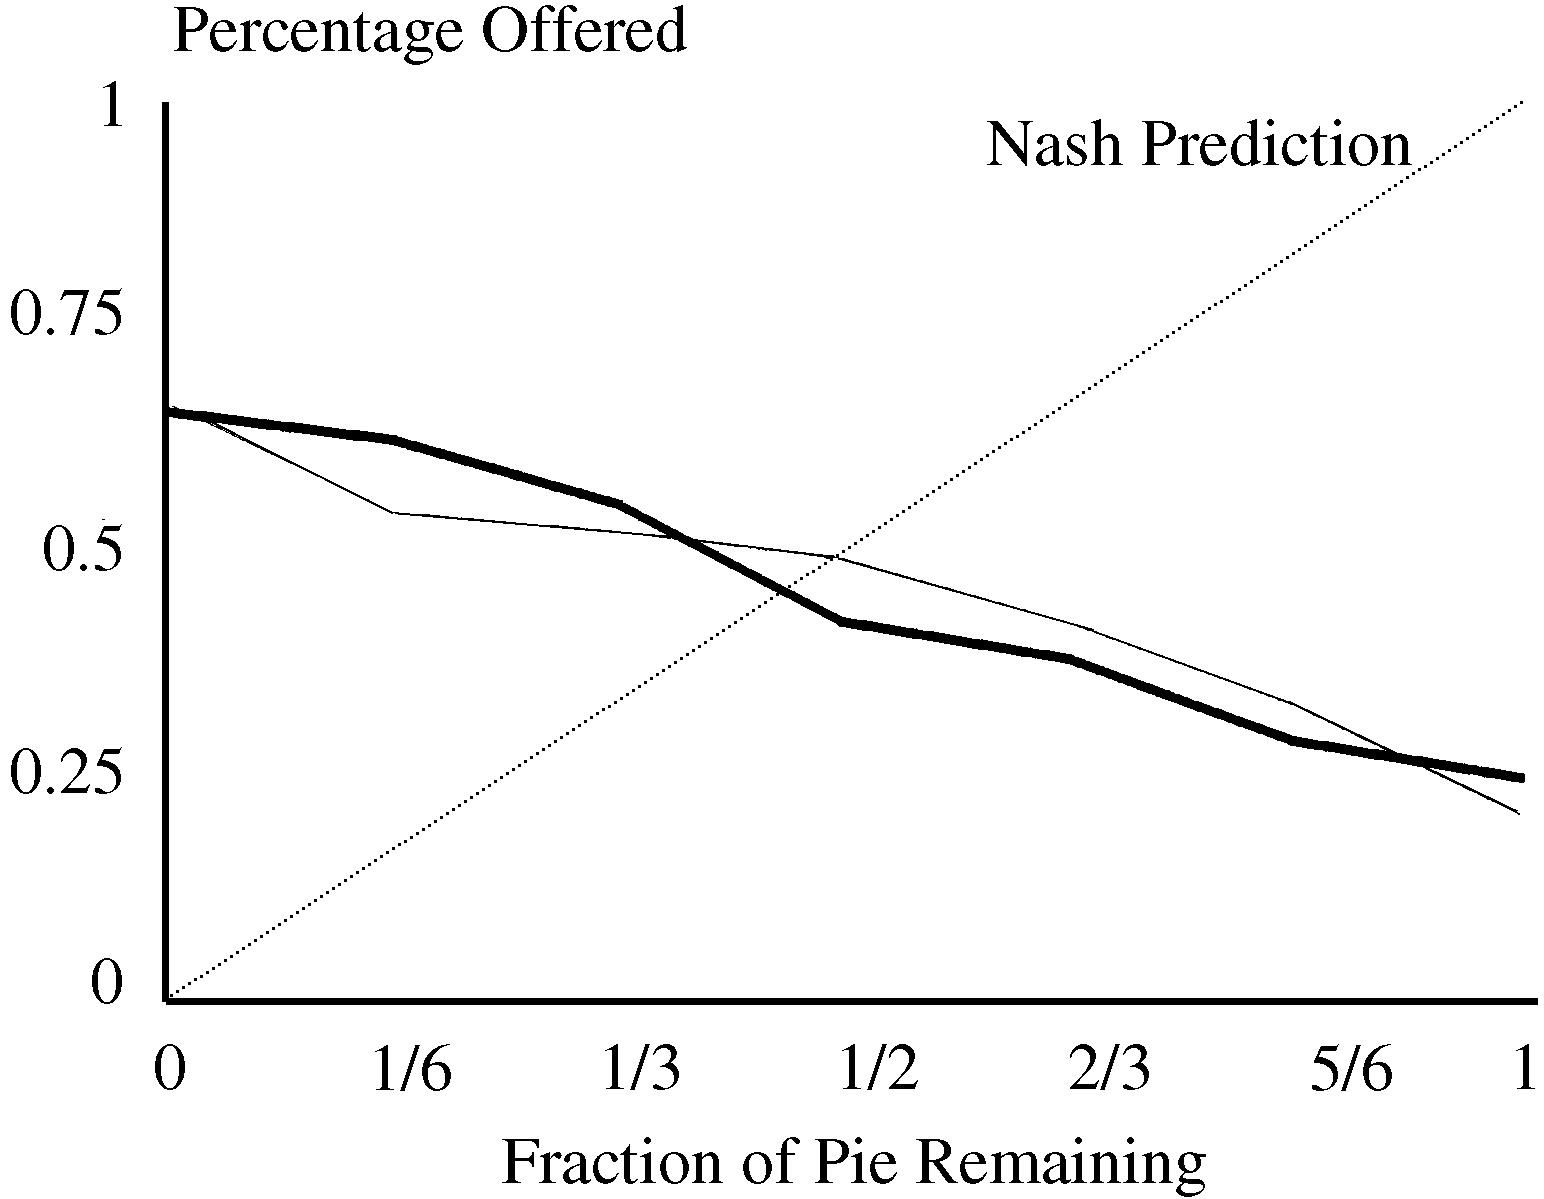
\includegraphics[width=0.7\textwidth]{holt.png}
      \end{center}

    \subsection{Hra investice}
      V této hře jsou dva hráči: investor a makléř. Investor na začátku dostane obdaření $X$ a může část $Y\leq X$
      odeslat makléři. Peníze jsou u makléře zhodnoceny vynásobením koeficientem $\alpha$. Makléř může investorovi
      zpět vrátit $Z\leq\alpha Y$. To si lze představit tak, že makléř pošle zpět zisk snížený o poplatek, nebo
      jednoduše vše ukradne. Celkový výdělek investora je $X-Y+Z$, makléře $\alpha Y-Z$.

      Za předpokladu sobeckosti a aplikací subgame-perfect rovnováhy zjistíme, že makléř nepošle nic zpátky. Investor
      s tím počítá, takže nic nepošle makléři. Není tedy vytvořen žádný ekonomický přebytek. Maximálního přebytku lze
      dosáhnout pokud investor pošle vše. Z tohoto pohledu už rozhodnutí makléře nic neovlivní.

      Berg et el. (1995) provedli tento experiment s parametry $X=\$10$, $\alpha=3$. Jedním z výsledků je tento graf:

      \begin{center}
        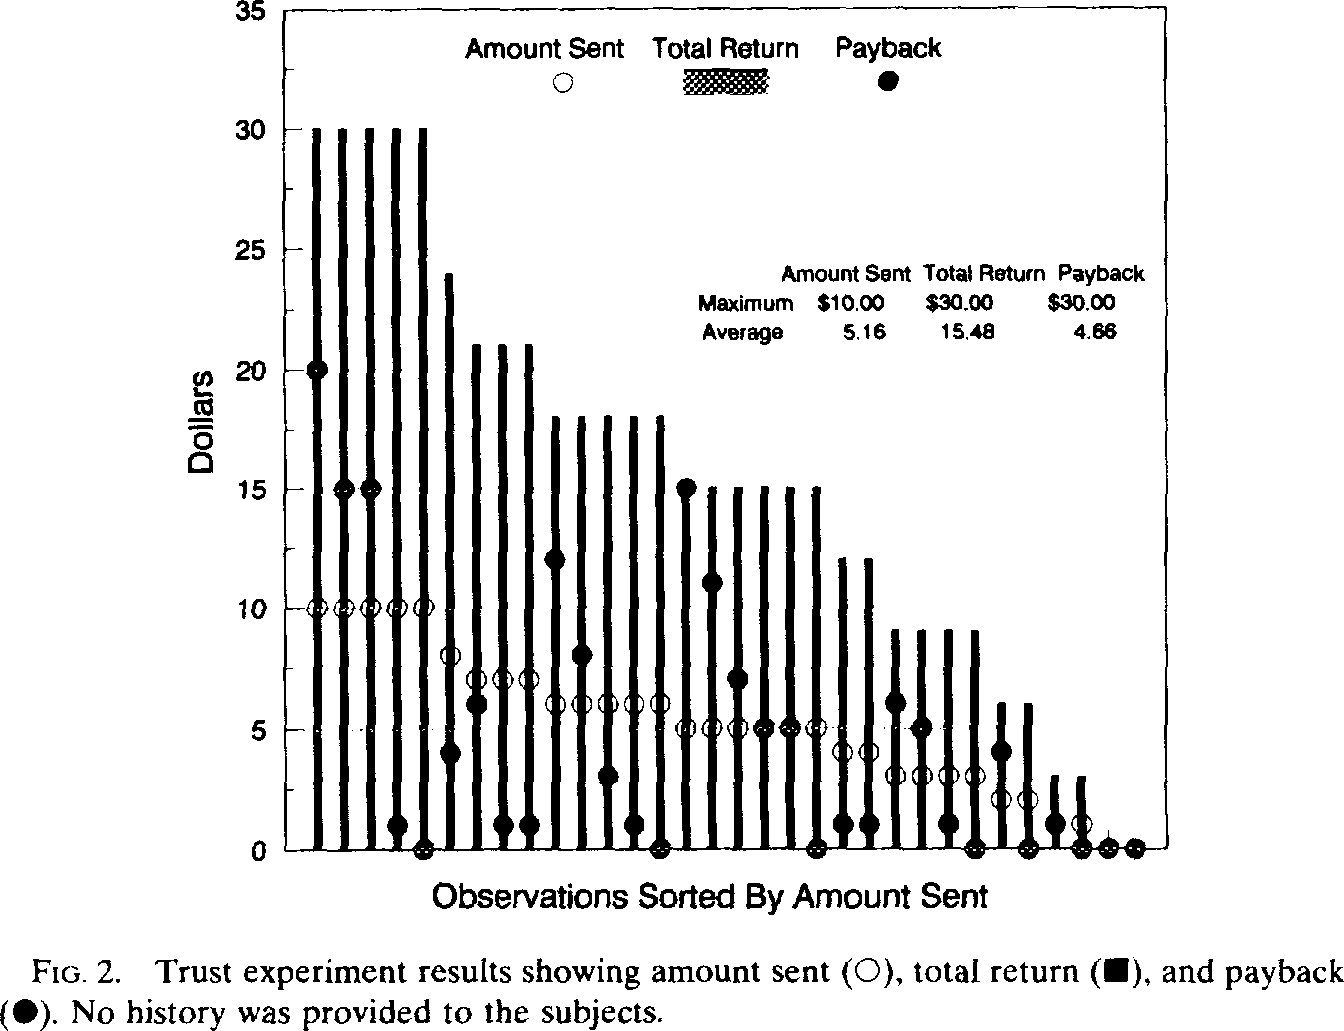
\includegraphics[width=0.6\textwidth]{berg.png}
      \end{center}


\end{document}
